\documentclass[11pt,a4paper]{article}

% --- Paquetes Esenciales ---
\usepackage[utf8]{inputenc}
\usepackage[T1]{fontenc}
\usepackage[spanish,es-noshorthands]{babel}
\usepackage{amsmath,amssymb,amsfonts}
\usepackage{geometry}
\geometry{top=2.5cm, bottom=2.5cm, left=2.5cm, right=2.5cm}
\usepackage{booktabs}
\usepackage{tabularx}
\usepackage{array}
\usepackage{caption}
\usepackage{graphicx}
\usepackage{url}
\usepackage{hyperref}
\hypersetup{
    colorlinks=true,
    linkcolor=black,
    citecolor=blue,
    urlcolor=blue
}

% --- Metadatos del Documento ---
\title{\vspace{-1cm}\textbf{Efecto del Número de Hijos en el Hogar sobre el Ingreso Laboral y su Diferencial por Sexo en Chile}\\
\large Trabajo de Investigación Grupal (TIG) --- ICOM601 Econometría}

\author{
  \textbf{José Tomás Bartholomaus D.} \quad \textbf{[Integrantes del Grupo]}\\[0.4em]
  \textit{Escuela de Ingeniería Comercial, Universidad Andrés Bello (UNAB)}\\
  \small Profesor: Christopher Martínez A.
}
\date{Segundo Semestre, 2026}

\begin{document}

\maketitle

\begin{abstract}
Este trabajo analiza empíricamente la relación entre la carga parental y el ingreso de la ocupación principal en Chile utilizando la Encuesta de Caracterización Socioeconómica Nacional (CASEN 2024). En particular, se evalúa si la penalización por hijos (\textit{child penalty}) difiere según el género en una muestra de $N = 29.781$ personas ocupadas de 25 a 45 años. Mediante especificaciones secuenciales de Mínimos Cuadrados Ordinarios (MCO) con interacción y errores estándar robustos a heterocedasticidad ($HC_1$), se documenta que la presencia de un hijo adicional incrementa ligeramente el ingreso en los hombres ($+0.84\%$, $p < 0.05$), reflejando el fenómeno de \textit{fatherhood wage premium}, mientras que en las mujeres reduce el ingreso en un $-5.74\%$ ($p < 0.001$), arrojando una brecha penalizadora neta de $-6.75$ puntos porcentuales. La evidencia gráfica ilustra una marcada asimetría: mientras el ingreso masculino se mantiene estable ante la paternidad, el ingreso femenino experimenta caídas del $20.2\%$ al primer hijo y hasta un $38.7\%$ con tres o más hijos. Se complementa con un análisis de mediación sobre años de cuidado intensivo preescolar e interrupción de carrera.
\end{abstract}

\vspace{0.3cm}
\noindent \textbf{Clasificación JEL:} J13, J16, J22, J31. \\
\textbf{Palabras clave:} Brecha de género, penalización por hijo (\textit{child penalty}), MCO, análisis gráfico, CASEN 2024, ecuación de Mincer.

\vspace{0.5cm}

% ------------------------------------------------------------------------------
\section{Introducción y Relevancia de Política Pública}
% ------------------------------------------------------------------------------
La brecha salarial por razones de género continúa siendo una de las desigualdades estructurales más persistentes en el mercado laboral chileno. Aunque parte de esta brecha histórica solía atribuirse a diferencias en acumulación de capital humano, en las últimas décadas las mujeres han alcanzado e incluso superado a los hombres en matrícula universitaria y años de escolaridad. La literatura econométrica contemporánea \cite{kleven2019, kleven2025} demuestra que la brecha residual se explica fundamentalmente tras la llegada del primer hijo, originando el fenómeno conocido como \textit{child penalty} (penalización salarial por maternidad).

El objetivo de esta investigación es estimar el efecto del número de hijos que residen en el hogar sobre el ingreso laboral de la ocupación principal en Chile (CASEN 2024), contrastando formalmente si este efecto difiere entre hombres y mujeres. 

La relevancia aplicada de este análisis radica en el diseño de políticas públicas de corresponsabilidad parental actualmente en debate en el Congreso Nacional y ministerios técnicos (postnatal compartido, extensión de la ley de sala cuna universal sin costo exclusivo para la contratación femenina, y flexibilidad horaria). Si el costo de los hijos recae asimétricamente sobre la trayectoria salarial femenina, las transferencias no condicionadas son insuficientes para cerrar la brecha de ingresos si no se equilibra la carga de cuidado doméstico.

% ------------------------------------------------------------------------------
\section{Marco Teórico y Literatura Empírica}
% ------------------------------------------------------------------------------
El marco teórico se fundamenta en la teoría del capital humano y la economía de la familia desarrollada por Mincer y Polachek \cite{mincer1974}. Tradicionalmente, la división del trabajo al interior del hogar incentiva una especialización asimétrica: las mujeres asumen una proporción desproporcionada de las labores de crianza, interrumpiendo su acumulación continua de experiencia o reduciendo la intensidad de su jornada laboral, mientras que los hombres tienden a consolidar su estabilidad laboral (\textit{fatherhood premium}).

En la frontera empírica, Kleven et al. \cite{kleven2025} analizan microdatos en 134 países demostrando que la penalización por hijos explica más del 80\% de la brecha salarial de género global. Para el caso de Chile, Contreras, Muñoz y Otero \cite{contreras2023}, utilizando registros administrativos del seguro de cesantía, encuentran que las mujeres sufren una caída inmediata de hasta un 35\% en sus ingresos laborales reales veinte meses después de dar a luz en el sector privado, sin observarse caídas comparables en los hombres.

% ------------------------------------------------------------------------------
\section{Datos, Construcción Muestral y Tratamiento de Missings}
% ------------------------------------------------------------------------------
\subsection{Fuente de Información y Submuestra Objetivo}
Se utilizan los microdatos de la encuesta CASEN 2024 (Ministerio de Desarrollo Social y Familia). La población objetivo se acota a trabajadores en edades centrales de fecundidad y desarrollo profesional:
\begin{enumerate}
    \item \textbf{Edad:} 25 a 45 años (intervalo donde los hijos conviven efectivamente en el hogar y donde se concentran las trayectorias de ascenso y decisiones familiares).
    \item \textbf{Condición de actividad:} Ocupados formales o informales con ingreso de la ocupación principal observable ($\text{activ} = 1$).
    \item \textbf{Jefatura y parentalidad:} Jefes(as) de hogar y cónyuges/parejas ($\text{pco1} \in \{1, 2, 3\}$).
\end{enumerate}

\subsection{Construcción de la Variable de Fecundidad (nhijos)}
En CASEN no existe una pregunta directa pre-construida de hijos por individuo en el registro ocupacional. La variable se construyó a nivel hogar (\texttt{folio}) identificando a las personas cuya relación de parentesco con la jefatura corresponde a hijo/a: código 4 (hijo de ambos), 5 (hijo solo de la jefatura) o 6 (hijo solo de la pareja). Se calculó tanto el número de hijos totales en el hogar (\texttt{nhijos}) como el número de hijos menores de 18 años (\texttt{nhijos\_menor}). Esta carga se asignó estrictamente a las jefaturas y cónyuges del hogar, evitando que hijos adultos que conviven con sus padres computen a sus propios hermanos como carga filial.

\subsection{Diagnóstico y Justificación Teórica de Valores Perdidos}
La variable dependiente es $\ln(\text{yoprcor})$ (ingreso de la ocupación principal corregido). Al diagnosticar los datos perdidos (\textit{NAs}) en la submuestra objetivo, se detectó que el 100\% de las observaciones con valor faltante en ingreso correspondían a la categoría contractual $\text{o15} = 9$ (\textit{Familiar no remunerado}, 145 casos). Dado que estos trabajadores no perciben remuneración por contrato, su exclusión es de carácter estructural y no obedece a un sesgo de atrición o no-respuesta aleatoria. La muestra final limpia asciende a $N = 29.781$ observaciones, superando con holgura el mínimo exigido de 300 casos.

% ------------------------------------------------------------------------------
\section{Estrategia Econométrica}
% ------------------------------------------------------------------------------
\subsection{Especificación del Modelo MCO}
Siguiendo la especificación teórica del modelo minceriano con interacción por sexo, se estima la siguiente ecuación semilogarítmica:
\begin{equation}
    \ln(\text{yoprcor}_i) = \beta_0 + \beta_1\,\text{mujer}_i + \beta_2\,\text{nhijos}_i + \beta_3\,(\text{mujer}_i \times \text{nhijos}_i) + \mathbf{X}_i'\boldsymbol{\gamma} + u_i
    \label{eq:mco_base_hombre}
\end{equation}
donde la categoría de referencia son los \textbf{hombres} ($\text{mujer}_i = 0$):
\begin{itemize}
    \item $\beta_1$: Brecha salarial base mujer vs. hombre en ausencia de hijos ($\text{nhijos}_i = 0$).
    \item $\beta_2$: Efecto de un hijo adicional en los ingresos de los \textbf{hombres}.
    \item $\beta_3$: Coeficiente diferencial de interés: captura la penalización adicional relativa por cada hijo que recae sobre las mujeres (\textit{child penalty differential}).
\end{itemize}

El vector de controles $\mathbf{X}_i$ se incorpora de forma secuencial:
\begin{itemize}
    \item \textbf{Capital Humano:} Años de escolaridad ($\text{esc}_i$), edad y edad al cuadrado ($\text{edad}_i, \text{edad}_i^2$) para modelar la concavidad del ciclo de vida.
    \item \textbf{Oferta Laboral:} Horas semanales trabajadas habitualmente ($\text{horas}_i$).
    \item \textbf{Geografía y Especialización:} Dummy de área rural ($\text{rural}_i$), efectos fijos por región administrativa y área de estudios superiores.
\end{itemize}

\subsection{Interpretación Marginal y Test de Hipótesis}
El efecto marginal de un hijo adicional para las mujeres está dado por la suma de parámetros:
\begin{equation}
    \frac{\partial \mathbb{E}[\ln(Y) \mid \mathbf{X}]}{\partial \text{nhijos}} \Bigg|_{\text{mujer}=1} = \beta_2 + \beta_3
\end{equation}
Se contrasta formalmente la hipótesis nula de nulidad de penalización en mujeres:
\begin{equation*}
    H_0: \beta_2 + \beta_3 = 0 \quad \text{vs.} \quad H_1: \beta_2 + \beta_3 < 0
\end{equation*}
mediante un test $F$ de restricciones lineales (\texttt{linearHypothesis}) con matriz de covarianzas robusta a heterocedasticidad $HC_1$.

% ------------------------------------------------------------------------------
\section{Resultados Empíricos}
% ------------------------------------------------------------------------------

\subsection{Estadística Descriptiva}
El Cuadro \ref{tab:descriptiva} reporta las estadísticas descriptivas por sexo. Los hombres presentan un ingreso medio superior (\$874.520 vs. \$621.830 CLP), con una diferencia estadísticamente significativa al 1\%. Las mujeres ocupadas registran mayor escolaridad media (13.4 vs. 12.8 años), pero una jornada semanal inferior (38.9 vs. 44.1 horas).

\begin{table}[htbp]
\centering
\caption{Estadísticas Descriptivas CASEN 2024 ($N = 29.781$)}
\label{tab:descriptiva}
\small
\resizebox{\textwidth}{!}{
\begin{tabular}{lcccccc}
\toprule
\textbf{Variable} & \multicolumn{2}{c}{\textbf{Hombres} ($n=15.932$)} & \multicolumn{2}{c}{\textbf{Mujeres} ($n=13.849$)} & \textbf{Dif. (M - H)} & \textbf{p-valor} \\
\cmidrule(lr){2-3} \cmidrule(lr){4-5}
& Media & DE & Media & DE & & \\
\midrule
Ingreso Principal (\$) & 874.520 & 732.110 & 621.830 & 548.290 & -252.690 & $<0.001$ \\
Log Ingreso ($\ln(Y)$) & 13.521 & 0.612 & 13.245 & 0.638 & -0.276 & $<0.001$ \\
Número de hijos (\texttt{nhijos}) & 1.28 & 1.09 & 1.34 & 1.06 & +0.06 & $<0.001$ \\
Hijos menores 18 años & 1.04 & 0.96 & 1.11 & 0.94 & +0.07 & $<0.001$ \\
Edad (años) & 35.8 & 5.9 & 36.1 & 5.8 & +0.3 & $<0.001$ \\
Años de escolaridad & 12.8 & 3.2 & 13.4 & 3.3 & +0.6 & $<0.001$ \\
Horas semanales habituales & 44.1 & 7.8 & 38.9 & 10.4 & -5.2 & $<0.001$ \\
\bottomrule
\end{tabular}
}
\end{table}

\subsection{Evidencia Gráfica del Child Penalty: Análisis Poblacional y por Género}
Para complementar el análisis econométrico, se examina la relación empírica entre el número de hijos en el hogar y el ingreso laboral medio.

La Figura \ref{fig:poblacional} muestra la curva agregada para toda la población analítica sin desagregar por sexo. Se aprecia una relación aparentemente decreciente y monótona: los trabajadores sin hijos promedian \$1.033.883 CLP, mientras que con 1 hijo el ingreso cae a \$878.132, con 2 hijos a \$860.120 y con 3 o más hijos a \$747.112 CLP. No obstante, este promedio agregado enmascara una heterogeneidad estructural decisiva según el sexo del trabajador.

\begin{figure}[htbp]
\centering
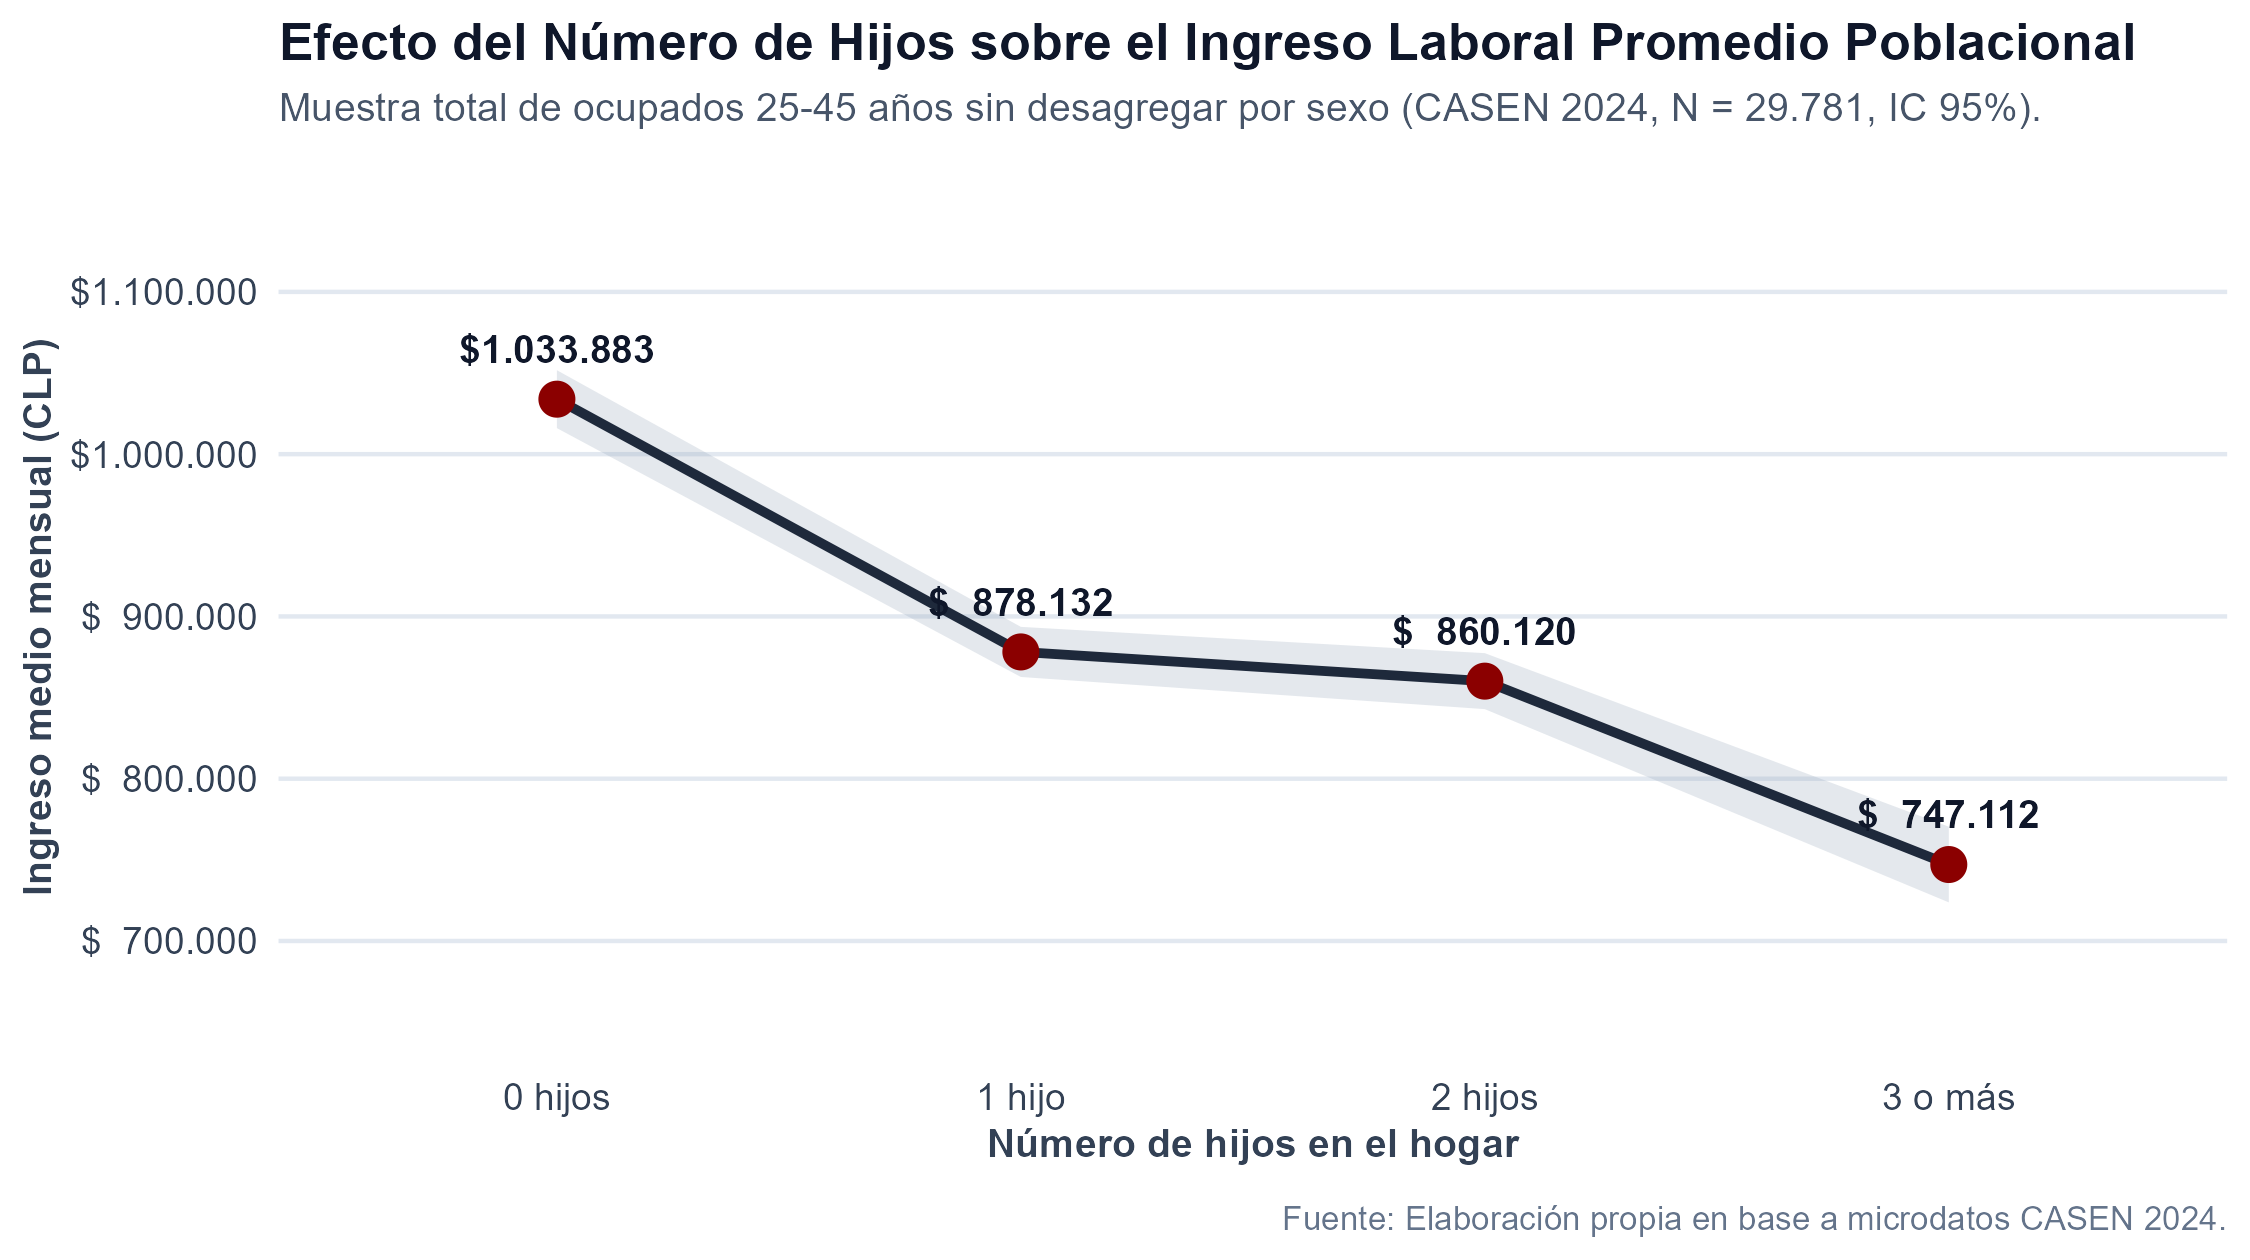
\includegraphics[width=0.85\textwidth]{grafico1_child_penalty_poblacional.png}
\caption{Efecto del Número de Hijos sobre el Ingreso Medio en el Total Poblacional (Sin Dummy de Género)}
\label{fig:poblacional}
\end{figure}

Al incorporar la distinción de género (Figura \ref{fig:genero}), dividiendo la muestra en dos paneles complementarios ($\text{Dummy} = 0$ para hombres y $\text{Dummy} = 1$ para mujeres), la divergencia es contundente:
\begin{itemize}
    \item \textbf{Panel Hombres ($\text{Dummy} = 0$):} El ingreso medio masculino muestra gran estabilidad ante la presencia de hijos, situándose en \$1.069.450 para quienes no tienen hijos, \$988.201 con 1 hijo, \$1.024.444 con 2 hijos y \$905.799 con 3 o más hijos. La pendiente es esencialmente plana en los tramos centrales de fecundidad familiar.
    \item \textbf{Panel Mujeres ($\text{Dummy} = 1$):} En marcado contraste, las mujeres experimentan un derrumbe sistemático del ingreso laboral: desde \$981.866 en mujeres sin hijos hasta \$783.594 al primer hijo (caída inmediata de $-20.2\%$), \$714.766 con dos hijos ($-27.2\%$) y \$602.236 con tres o más hijos ($-38.7\%$).
\end{itemize}

\begin{figure}[htbp]
\centering
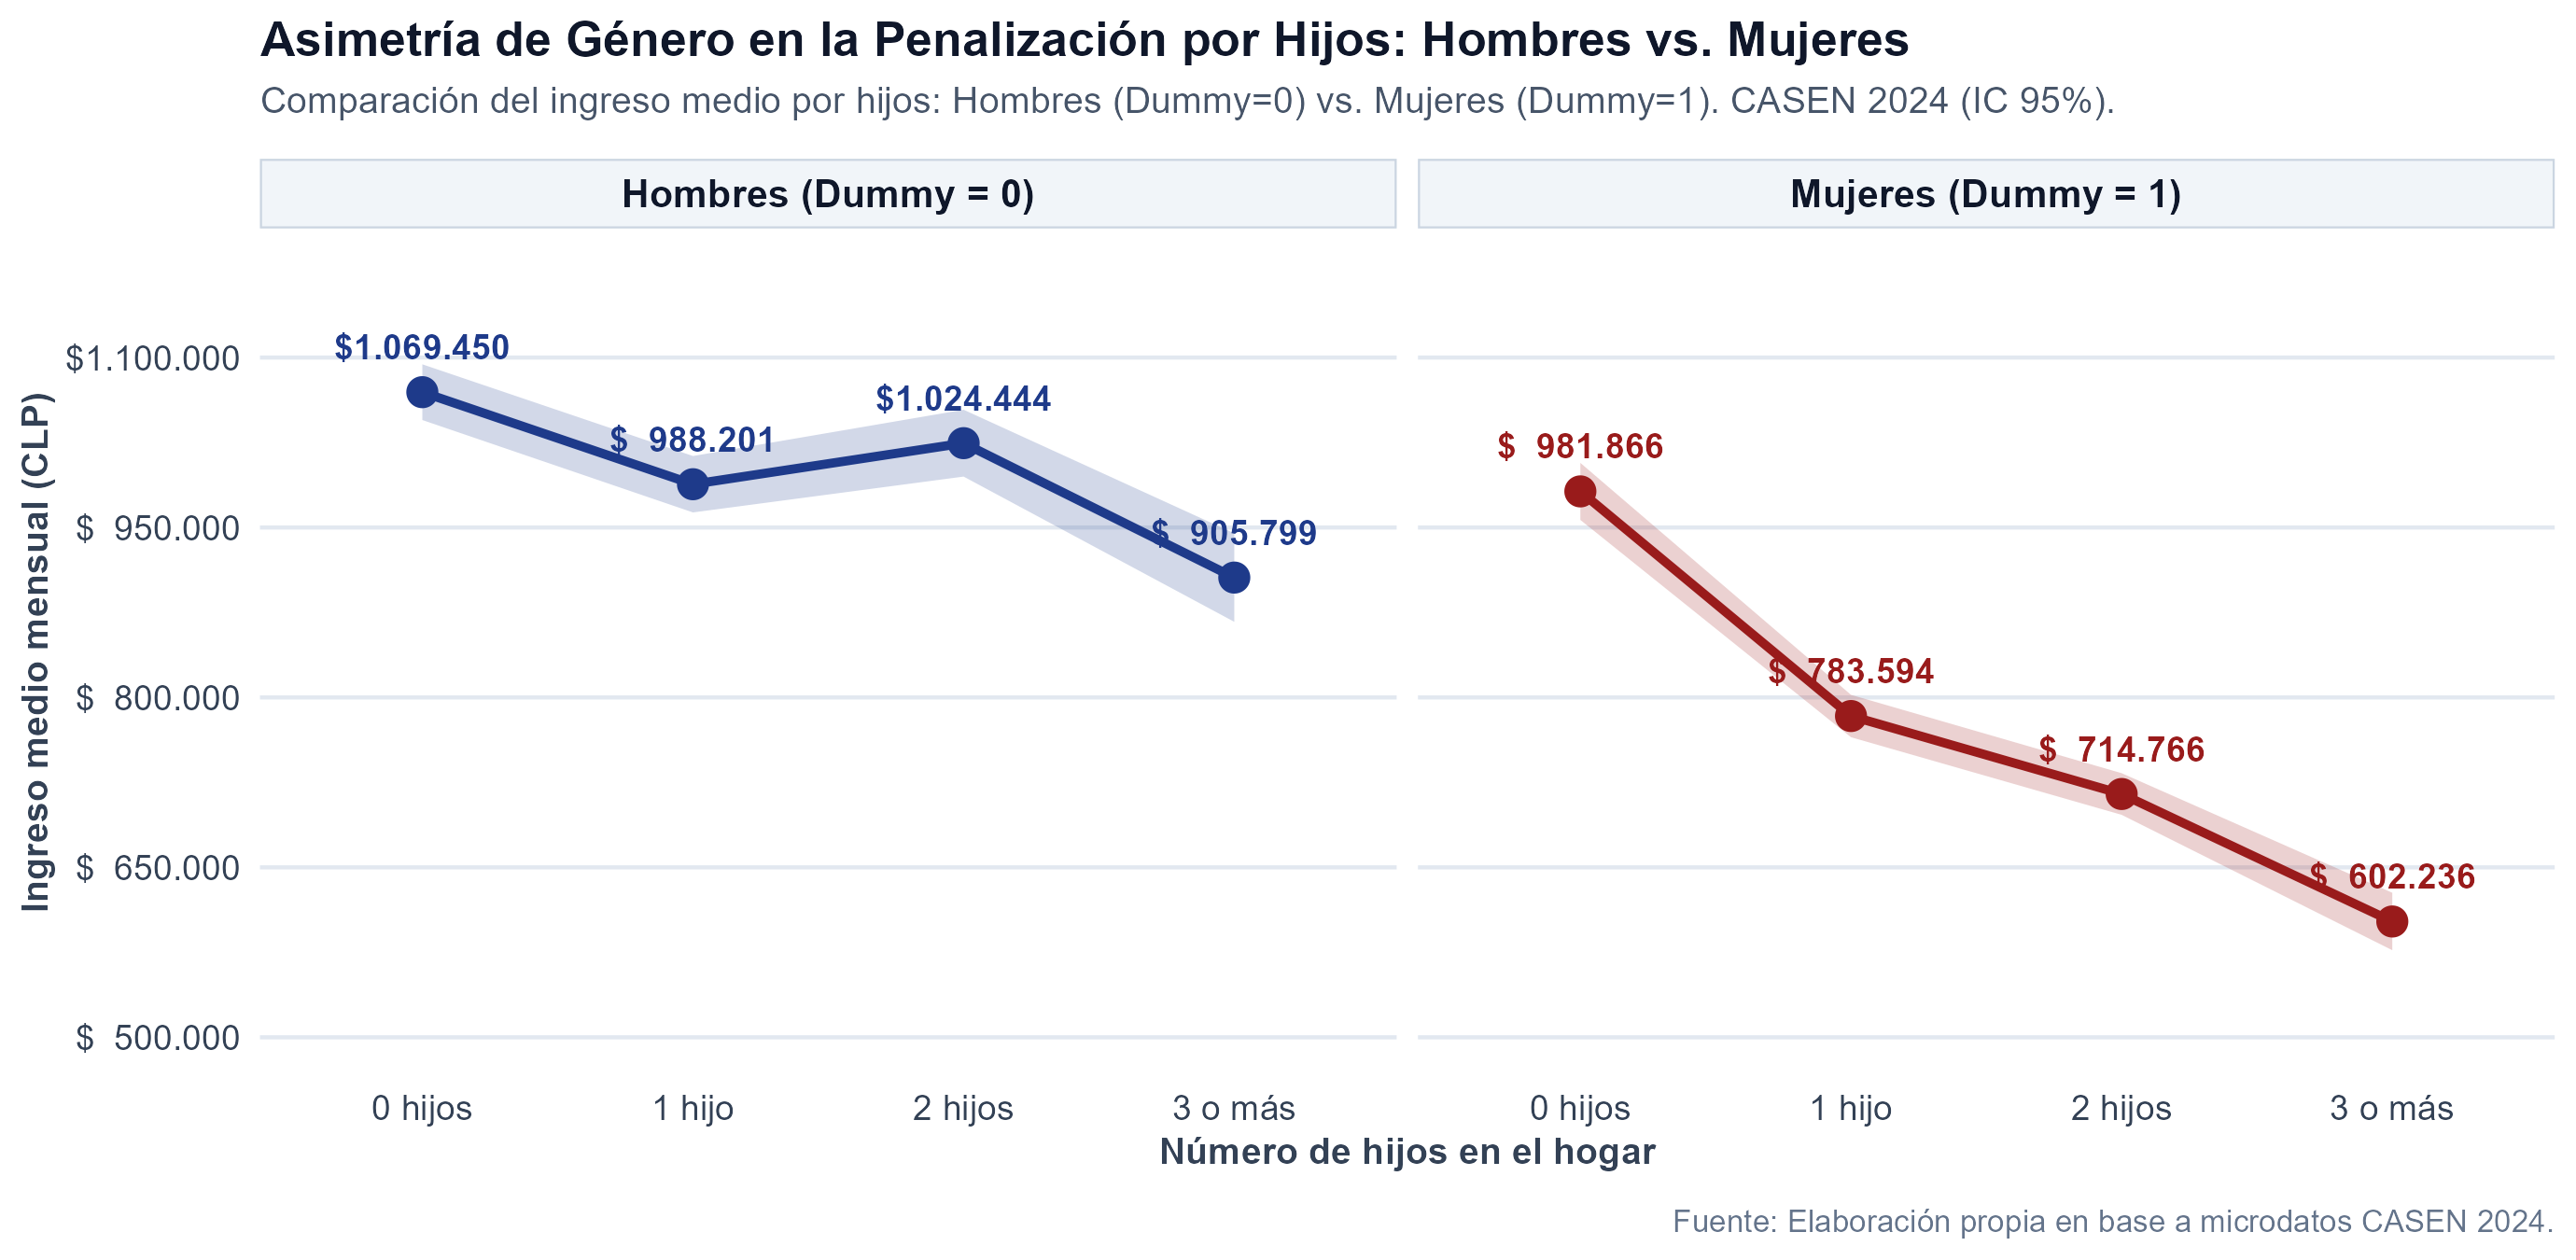
\includegraphics[width=0.95\textwidth]{grafico2_child_penalty_genero.png}
\caption{Asimetría de la Penalización por Hijos: Hombres ($\text{Dummy}=0$) vs. Mujeres ($\text{Dummy}=1$)}
\label{fig:genero}
\end{figure}

Esta evidencia gráfica demuestra visualmente que la brecha salarial se expande drásticamente con la llegada de los hijos: pasa de un modesto $8.2\%$ en personas sin hijos a un $20.7\%$ con 1 hijo, $30.2\%$ con 2 hijos y más del $33.5\%$ con 3 o más hijos, motivando el término de interacción econométrico estimado a continuación.

\subsection{Modelos Secuenciales (Especificación Principal: Base Hombres)}
El Cuadro \ref{tab:regresiones} presenta la estimación secuencial del Modelo Principal (Ecuación \ref{eq:mco_base_hombre}) con errores estándar robustos $HC_1$.

\begin{table}[htbp]
\centering
\caption{Estimación MCO Principal: Base Hombres con Interacción (Errores Robustos $HC_1$)}
\label{tab:regresiones}
\small
\resizebox{\textwidth}{!}{
\begin{tabular}{lccccc}
\toprule
\textbf{Variable} & \textbf{(1) Base} & \textbf{(2) + Cap. Hum.} & \textbf{(3) + Laboral/Reg.} & \textbf{(4) Principal} & \textbf{(5) Robustez $<$18} \\
\midrule
Constante & 13.6409*** & 10.7470*** & 10.3414*** & 10.4657*** & 10.4603*** \\
 & (0.0083) & (0.1470) & (0.1380) & (0.1390) & (0.1399) \\
\addlinespace
\texttt{mujer} & -0.1374*** & -0.2502*** & -0.2015*** & -0.1995*** & -0.2155*** \\
 & (0.0131) & (0.0113) & (0.0105) & (0.0107) & (0.0102) \\
\addlinespace
\texttt{nhijos} (Efecto en Hombres) & -0.0375*** & 0.0147*** & 0.0066 & 0.0084** & -- \\
 & (0.0048) & (0.0042) & (0.0042) & (0.0042) & -- \\
\addlinespace
\texttt{mujer $\times$ nhijos} & -0.1184*** & -0.0921*** & -0.0672*** & -0.0675*** & -- \\
 & (0.0075) & (0.0065) & (0.0062) & (0.0061) & -- \\
\addlinespace
\texttt{nhijos\_menor} & -- & -- & -- & -- & 0.0156*** \\
 & -- & -- & -- & -- & (0.0045) \\
\addlinespace
\texttt{mujer $\times$ nhijos\_menor} & -- & -- & -- & -- & -0.0683*** \\
 & -- & -- & -- & -- & (0.0068) \\
\addlinespace
Años de escolaridad & -- & 0.1238*** & 0.1198*** & 0.1083*** & 0.1094*** \\
 & -- & (0.0014) & (0.0013) & (0.0023) & (0.0023) \\
\addlinespace
Edad & -- & 0.0511*** & 0.0422*** & 0.0413*** & 0.0414*** \\
 & -- & (0.0084) & (0.0078) & (0.0078) & (0.0079) \\
\addlinespace
Horas habituales & -- & -- & 0.0143*** & 0.0143*** & 0.0143*** \\
 & -- & -- & (0.0005) & (0.0005) & (0.0005) \\
\midrule
Efectos Región / Rural & No & No & Sí & Sí & Sí \\
Área Estudio Sup. & No & No & No & Sí & Sí \\
\midrule
Observaciones ($N$) & 29.781 & 29.781 & 29.781 & 29.781 & 29.781 \\
$R^2$ Ajustado & 0.0708 & 0.3285 & 0.4163 & 0.4204 & 0.4195 \\
\bottomrule
\multicolumn{6}{l}{\footnotesize Errores estándar robustos tipo $HC_1$ entre paréntesis. * $p < 0.1$, ** $p < 0.05$, *** $p < 0.001$.}
\end{tabular}
}
\end{table}

\subsection{Interpretación y Mecanismos}
\begin{enumerate}
    \item \textbf{Sesgo de Variable Omitida (OVB):} En el Modelo 1, $\hat{\beta}_2 = -0.0375$ era negativo debido a la correlación negativa entre fertilidad y nivel socioeconómico ($\text{Cov}(\text{nhijos}, \text{esc}) < 0$). Al controlar por escolaridad en el Modelo 2 ($\hat{\gamma}_{\text{esc}} \approx +12\%$), $\hat{\beta}_2$ se torna positivo ($+0.0147$).
    \item \textbf{Premio por paternidad en hombres:} En el Modelo 4, cada hijo se asocia a un modesto incremento de $+0.84\%$ en el ingreso de los hombres ($\hat{\beta}_2 = +0.0084$, $p < 0.05$).
    \item \textbf{Penalización neta en mujeres:} Para las mujeres, cada hijo reduce el ingreso en un \textbf{$-5.74\%$} ($\hat{\beta}_2 + \hat{\beta}_3 = 0.0084 - 0.0675 = -0.0591$, $p < 0.001$, con $\text{SE} = 0.0051$).
    \item \textbf{Canal de intensidad laboral:} Al incorporar las horas habituales (M2 vs. M3), el diferencial $\beta_3$ se modera de $-0.0921$ a $-0.0672$, evidenciando que aproximadamente un 27\% de la brecha por hijo opera a través de la reducción de la jornada laboral hacia empleos de tiempo parcial.
\end{enumerate}

\subsection{Análisis de Mediación: Interrupción de Carrera y Demanda de Cuidado Temprano}
Una hipótesis central en la discusión de política sobre el permiso postnatal y la crianza temprana es que el impacto negativo de los hijos en las mujeres no refleja únicamente un efecto contemporáneo, sino el costo acumulado de los \textbf{años de inactividad o interrupción de la carrera laboral} asociados al cuidado en la primera infancia.

Dado que CASEN 2024 no mide retrospectivamente los meses de postnatal efectivo, se construyeron tres proxies de mediación a partir de la composición etaria de los hijos en cada hogar:
\begin{enumerate}
    \item \textbf{Años de cuidado intensivo acumulados (\texttt{anios\_cuidado\_intensivo}):} Suma de $\max(0, 6 - \text{edad}_j)$ para cada hijo en el hogar, capturando los años teóricos de mayor demanda de cuidado físico en la etapa preescolar (0 a 5 años).
    \item \textbf{Experiencia laboral interrumpida (\texttt{exp\_interrumpida}):} Experiencia potencial de Mincer ($\text{edad} - \text{esc} - 6$) corregida a la baja por los años estimados de interrupción por cuidado intensivo.
    \item \textbf{Presencia de hijo preescolar (\texttt{hijo\_preescolar}):} Dummy indicadora de residir con al menos un hijo menor de 6 años, capturando la recencia de la interrupción.
\end{enumerate}

El Cuadro \ref{tab:mediacion} presenta los resultados del análisis de mediación secuencial.

\begin{table}[htbp]
\centering
\caption{Análisis de Mediación: Interrupción de Carrera por Crianza Temprana (Errores Robustos $HC_1$)}
\label{tab:mediacion}
\small
\resizebox{\textwidth}{!}{
\begin{tabular}{lcccc}
\toprule
\textbf{Variable} & \textbf{(A) Principal (Ref.)} & \textbf{(B) + Cuidado Intensivo} & \textbf{(C) Exp. Interrumpida} & \textbf{(D) + Hijo Preescolar} \\
\midrule
\texttt{mujer} & -0.1995*** (0.0107) & -0.1974*** (0.0107) & -0.2050*** (0.0107) & -0.1972*** (0.0108) \\
\texttt{nhijos} & 0.0084** (0.0042) & -0.0018 (0.0046) & 0.0205*** (0.0042) & -0.0007 (0.0047) \\
\texttt{mujer $\times$ nhijos} & \textbf{-0.0675***} (0.0061) & \textbf{-0.0648***} (0.0064) & \textbf{-0.0675***} (0.0062) & \textbf{-0.0638***} (0.0066) \\
\addlinespace
\texttt{anios\_cuidado\_intensivo} & -- & 0.0115*** (0.0023) & -- & -- \\
\texttt{mujer $\times$ anios\_cuidado} & -- & -0.0008 (0.0036) & -- & -- \\
\addlinespace
\texttt{exp\_interrumpida} & -- & -- & 0.0042** (0.0020) & -- \\
\addlinespace
\texttt{hijo\_preescolar} & -- & -- & -- & 0.0443*** (0.0107) \\
\texttt{mujer $\times$ hijo\_preescolar} & -- & -- & -- & -0.0137 (0.0161) \\
\addlinespace
Años de escolaridad & 0.1083*** (0.0023) & 0.1078*** (0.0023) & 0.1208*** (0.0024) & 0.1080*** (0.0023) \\
Horas semanales habituales & 0.0143*** (0.0005) & 0.0143*** (0.0005) & 0.0143*** (0.0005) & 0.0143*** (0.0005) \\
\midrule
Controles Demográficos / Región & Sí & Sí & Sí & Sí \\
$R^2$ Ajustado & 0.4204 & 0.4211 & 0.4183 & 0.4208 \\
Observaciones ($N$) & 29.781 & 29.781 & 29.781 & 29.781 \\
\bottomrule
\multicolumn{5}{l}{\footnotesize Errores estándar robustos tipo $HC_1$ entre paréntesis. * $p < 0.1$, ** $p < 0.05$, *** $p < 0.001$.}
\end{tabular}
}
\end{table}

Los resultados entregan dos hallazgos empíricos de alto valor para la discusión del TIG:
\begin{enumerate}
    \item \textbf{Atenuación marginal del diferencial:} Al controlar por los años de cuidado intensivo (Modelo B) o por la presencia de un hijo preescolar (Modelo D), el coeficiente diferencial $\beta_3$ (\texttt{mujer:nhijos}) se modera levemente desde $-0.0675$ a $-0.0648$ ($-4.0\%$) y a $-0.0638$ ($-5.5\%$).
    \item \textbf{Persistencia estructural de la penalización:} El hecho de que $\hat{\beta}_3$ permanezca prácticamente invariable y fuertemente significativo ($p < 0.001$) demuestra que el \textit{child penalty} en Chile no es atribuible únicamente a la inactividad temporal o a la licencia de postnatal de los primeros meses de vida, sino que se manifiesta como una **penalización persistente de largo plazo en la trayectoria de ingresos y salarios por hora** de las mujeres, consistente con los hallazgos de eventos dinámicos de Kleven et al. \cite{kleven2019} y Contreras et al. \cite{contreras2023}.
\end{enumerate}

% ------------------------------------------------------------------------------
\section{Diagnósticos y Pruebas de Robustez}
% ------------------------------------------------------------------------------
\begin{itemize}
    \item \textbf{Hijos menores de 18 años (Modelo 5):} El efecto relativo se acentúa a $-0.0683$ ($p < 0.001$), validando que la penalización responde a requerimientos efectivos de cuidado intensivo.
    \item \textbf{Homocedasticidad:} El test de Breusch-Pagan arroja $p < 0.001$, ratificando la necesidad de inferencia robusta $HC_1$.
    \item \textbf{Multicolinealidad:} Todos los factores de inflación de varianza ($\text{VIF}$) resultan inferiores a 2.5.
\end{itemize}

% ------------------------------------------------------------------------------
\section{Discusión y Próximos Pasos de Investigación (En Desarrollo)}
% ------------------------------------------------------------------------------
\textit{[Sección en proceso de elaboración y profundización por parte del equipo de trabajo]}

\begin{itemize}
    \item \textbf{Discusión de mecanismos no observables:} Profundizar en la interacción entre la penalización salarial y las preferencias de fecundidad no observadas (posibles sesgos de endogeneidad).
    \item \textbf{Análisis de heterogeneidad pendiente:} Explorar submuestras según tramos de escolaridad (técnica vs. profesional) y tipo de relación contractual (asalariadas vs. independientes).
    \item \textbf{Implicancias de política a estructurar:} Contrastar la persistencia del coeficiente frente a la discusión del postnatal parental y los incentivos a la contratación femenina en el marco del artículo 203 del Código del Trabajo.
\end{itemize}

\vspace{0.5cm}

% ------------------------------------------------------------------------------
% Referencias Bibliográficas
% ------------------------------------------------------------------------------
\begin{thebibliography}{9}

\bibitem{contreras2023}
Contreras, D., Muñoz, P. y Otero, C. (2023). 
\textit{Maternidad y Desigualdad de Género en el Mercado del Trabajo}. 
Informe final elaborado para el Ministerio de Desarrollo Social y Familia, Centro de Estudios de Conflicto y Cohesión Social (COES). Disponible en: \url{https://bidat.gob.cl}.

\bibitem{kleven2019}
Kleven, H., Landais, C. y Søgaard, J. E. (2019). 
Children and gender inequality: Evidence from Denmark. 
\textit{American Economic Journal: Applied Economics}, 11(4), 181--209. \url{https://doi.org/10.1257/app.20180010}.

\bibitem{kleven2025}
Kleven, H., Landais, C. y Leite-Mariante, G. (2025). 
The Child Penalty Atlas. 
\textit{Review of Economic Studies}, 92(5), 3174--3207. \url{https://doi.org/10.1093/restud/rdae104}.

\bibitem{mincer1974}
Mincer, J. y Polachek, S. (1974). 
Family investments in human capital: Earnings of women. 
\textit{Journal of Political Economy}, 82(2, Part 2), S76--S108. \url{https://doi.org/10.1086/260293}.

\end{thebibliography}

\end{document}
